\documentclass[aspectratio=169,11pt]{beamer}
\usetheme{default}
\usecolortheme{whale}
\setbeamertemplate{navigation symbols}{}
\setbeamertemplate{footline}[frame number]
\setbeamerfont{frametitle}{series=\bfseries}
\setbeamercolor{frametitle}{fg=white,bg=structure}
\usepackage{graphicx}
\usepackage{tikz}
\usetikzlibrary{arrows.meta,positioning}
\usepackage{amsmath}
\usepackage{booktabs}
\usepackage{colortbl}
\setbeamertemplate{itemize items}[circle]

% ---- toggle notes: `\setbeameroption{show notes}` for the notes build ----

\title{\textbf{Learning to Route}}
\subtitle{An RL-Gated Policy for Hierarchical Speculative Decoding}
\author{viasd-rl}
\date{\today}

\begin{document}

\begin{frame}\titlepage\end{frame}
\note{
One breath: speculative decoding speeds up LLMs; VIA-SD makes it smarter with a slim middle verifier
--- but it routes between tiers with \emph{hand-picked thresholds}. We recast that routing as a
learned decision problem and get a Pareto improvement over the hand-tuned baseline.
}

% =====================================================================
\begin{frame}{Overview}
\textbf{We introduce the first reinforcement-learned routing policy for hierarchical speculative decoding.}
\vspace{3pt}

{\footnotesize Speculative decoding accelerates LLM inference; VIA-SD adds a slim intermediate verifier but
routes between tiers with \emph{hand-tuned confidence thresholds}.}
\vspace{4pt}

We present \textbf{three key innovations}:
\begin{enumerate}
  \item a \textbf{learned per-token gating policy} that recasts tier-routing as a sequential decision problem --- a tiny $q$-free MLP replaces the fixed thresholds;
  \item a \textbf{quality--cost reward} that balances matching the target model against expensive-call latency;
  \item a \textbf{per-token RL formulation} with principled credit assignment (REINFORCE $\to$ GRPO $\to$ per-token advantage).
\end{enumerate}
\vspace{2pt}
{\footnotesize We challenge the assumption that hierarchical verification needs hand-tuned thresholds: a learned gate
\textbf{Pareto-dominates} the fixed-threshold baseline, recovering \emph{lossless} quality at a fraction of the expensive verifier calls.}
\end{frame}
\note{
This is the abstract. Strong claim first: the first \emph{learned} router for hierarchical
speculative decoding. Then the gap: VIA-SD's tiers are routed by hand-tuned thresholds. Then our
three contributions --- the learned gate, the reward that trades quality against cost, and the RL
training with per-token credit assignment. And the thesis we challenge: that you need to hand-tune
thresholds at all. Spend the rest of the talk unpacking these three.
}

% =====================================================================
\begin{frame}{The bottleneck: LLM decoding is slow and sequential}
\begin{itemize}
  \item Each token \textbf{streams the entire model} from memory --- inference is \emph{memory-bandwidth bound}.
  \item \textbf{Speculative decoding (SD):} a cheap \emph{drafter} guesses several tokens; the big \emph{verifier} checks them in \textbf{one parallel pass}.
  \item Accepted guesses $\Rightarrow$ many tokens per expensive forward. \textbf{Lossless}, $\sim$\textbf{1.4$\times$} wall-clock.
  \item The one lever: the \textbf{acceptance rate} --- every rejected token forces a full-model step.
\end{itemize}
\end{frame}
\note{
Frame the cost. Generating each token reads every weight from memory --- the sequential bottleneck
behind latency and serving cost. SD's trick: a small drafter proposes the next few tokens, and the
big verifier checks them all in one parallel forward. Accepted tokens ride free; the output is
identical to normal decoding. ~1.4x wall-clock on our pair. The whole game is the acceptance rate.
}

% =====================================================================
\begin{frame}{VIA-SD improves on vanilla SD}
\begin{columns}
\begin{column}{0.52\textwidth}
\textbf{Vanilla SD} --- binary per token:
\begin{itemize}\item \textsc{accept} drafter, or \textsc{reject} $\to$ full model $q$.\end{itemize}
\vspace{3pt}
\textbf{VIA-SD} --- adds a \textbf{slim middle verifier $q'$} ($q$ with $\sim$45\% of layers skipped):
\begin{itemize}
  \item \textsc{accept} \;|\; \textsc{regenerate} ($q'$) \;|\; \textsc{escalate} ($q$).
  \item ``Middle-zone'' tokens handled \emph{cheaply} by $q'$ $\Rightarrow$ fewer full-model calls.
\end{itemize}
\end{column}
\begin{column}{0.48\textwidth}
\centering
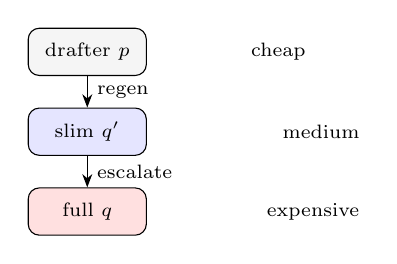
\begin{tikzpicture}[font=\scriptsize,>=Stealth,node distance=4mm,
  m/.style={draw,rounded corners,minimum width=15mm,minimum height=6mm,align=center}]
\node[m,fill=gray!8] (p) {drafter $p$};
\node[m,below=of p,fill=blue!10] (qp) {slim $q'$};
\node[m,below=of qp,fill=red!12] (q) {full $q$};
\draw[->] (p)--(qp) node[midway,right]{regen}; \draw[->] (qp)--(q) node[midway,right]{escalate};
\node[right=12mm of p] {cheap}; \node[right=16mm of qp] {medium}; \node[right=14mm of q] {expensive};
\end{tikzpicture}
\end{column}
\end{columns}
\end{frame}
\note{
Vanilla SD is all-or-nothing. VIA-SD's insight: many ``rejected'' tokens are borderline. So it adds a
cheaper middle judge --- the same big model with ~45\% of layers skipped --- and makes a three-way
choice: accept the drafter, regenerate with q-prime, or escalate to the full model. Borderline tokens
go to the cheap tier, so you call the full model far less. But how does it \emph{decide}? Next slide.
}

% =====================================================================
\begin{frame}{\dots but it routes with \emph{hand-picked thresholds}}
\begin{block}{VIA-SD's routing rule}
\centering Two fixed confidence thresholds on $q'$:\quad $\boxed{\alpha_1 = 0.5}$\quad $\boxed{\alpha_2 = 0.3}$
\end{block}
\vspace{2pt}
\begin{itemize}
  \item \textbf{Global \& static} --- one cutoff for every token and context.
  \item \textbf{Brittle} --- must be re-tuned per model and task.
  \item \textbf{Sub-optimal} --- even fully swept, accuracy peaks at $\le 0.50$ on our setup.
\end{itemize}
\vspace{3pt}
\centering\textit{Choosing a tier \emph{per token} is a sequential, context-dependent decision --- so \textbf{learn} it.}
\end{frame}
\note{
The opening. VIA-SD's three-way choice is two hand-picked numbers, 0.5 and 0.3 --- global, static,
context-blind, and re-tuned per model/task. Even sweeping all nine configs, accuracy caps at 0.50 on
our setup. But picking a tier per token from context is exactly a sequential decision problem. So
learn the policy. That sets up our three innovations.
}

% =====================================================================
\section{Method}
\begin{frame}{Innovation 1/3 --- a learned per-token gating policy (MDP)}
\begin{columns}
\begin{column}{0.56\textwidth}
\small Recast tier-routing as a \textbf{Markov decision process}:
\begin{itemize}
  \item \textbf{State} $s_t$: $q$-free features --- drafter/$q'$ confidence, agreement, $\mathrm{KL}(p\Vert q')$, position.
  \item \textbf{Action} $a_t\in\{$accept, regenerate, escalate$\}$.
  \item \textbf{Policy} $\pi_\theta(a_t\mid s_t)$: a tiny MLP.
\end{itemize}
\vspace{3pt}
\footnotesize Key property: $q$ is consulted only to \emph{score} at train time --- \textbf{never} a gate input,
so the gate is free to run at inference.
\end{column}
\begin{column}{0.44\textwidth}
\centering
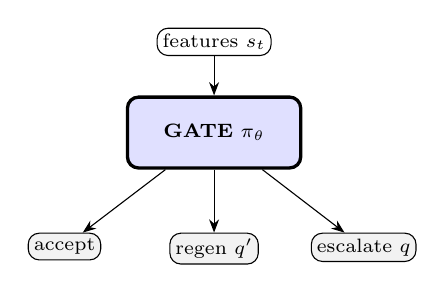
\begin{tikzpicture}[font=\scriptsize,>=Stealth,
  g/.style={draw,very thick,fill=blue!12,rounded corners,minimum width=22mm,minimum height=9mm,align=center},
  a/.style={draw,rounded corners,fill=gray!10,align=center,inner sep=2pt},
  io/.style={draw,rounded corners,align=center,inner sep=2pt}]
\node[io] (f) {features $s_t$};
\node[g,below=5mm of f] (g) {\textbf{GATE} $\pi_\theta$};
\node[a,below=8mm of g,xshift=-19mm] (x){accept};
\node[a,below=8mm of g] (y){regen $q'$};
\node[a,below=8mm of g,xshift=19mm] (z){escalate $q$};
\draw[->](f)--(g);\draw[->](g)--(x);\draw[->](g)--(y);\draw[->](g)--(z);
\end{tikzpicture}
\end{column}
\end{columns}
\end{frame}
\note{
Innovation one: the learned gate. We formalize routing as an MDP. The state is a handful of cheap
features --- drafter and q-prime confidence, whether they agree, their KL, position in the block. The
action is the tier. The policy is a tiny MLP. The crucial design choice: the features are q-free, so
the full model is used only to compute rewards during training; at inference the gate decides without
ever running q. That makes it free to deploy --- no extra serving model.
}

% =====================================================================
\begin{frame}{Innovation 2/3 --- a quality--cost reward}
\textbf{Two ingredients per token:}
\begin{align*}
\text{quality:}\quad & \text{match}_t = \mathbf{1}\big[\hat y_t = \arg\max\nolimits_v q(v\mid x_{<t})\big] \\[-1pt]
\text{cost:}\quad & \text{cost}_t = \big(t_{p_1} + t_{q'}/\gamma + \mathbf{1}[\textsc{escalate}]\,t_q\big)\big/\,t_{q_1}
\end{align*}
\textbf{Reward} (cost in units of one full-model step):
\begin{align*}
\text{trajectory:}\ & R = \overline{\text{match}} - \lambda\,\overline{\text{cost}}\ (+\,r_c\,\text{correct})
\qquad\qquad
\text{per-token:}\ r_t = \text{match}_t - \lambda\,\text{cost}_t
\end{align*}
\centering\footnotesize $\lambda$ is the \textbf{quality$\leftrightarrow$speed knob}; \texttt{match} is a \emph{dense}
proxy for the sparse true objective (final-answer correctness).
\end{frame}
\note{
Innovation two: the reward. Quality is whether the emitted token matches what the full model would
greedily produce --- computed by running q at train time only. Cost is the per-action latency:
drafter step, plus the slim q-prime amortized over the block, plus the full model only if we
escalate, all normalized by one full-model step. The reward subtracts lambda times cost from match;
lambda is the quality-versus-speed knob. We use both a trajectory form and a per-token form. One
caveat we measured: match is a dense proxy --- 98.5\% token match still leaves ~0.72 final accuracy,
because a few token slips derail the chain.
}

% =====================================================================
\begin{frame}{Innovation 3/3 --- per-token RL with credit assignment}
\textbf{Policy gradient} (all variants, $+\,\eta\,\mathcal{H}[\pi_\theta]$ entropy):
\[
\nabla_\theta J = \mathbb{E}\Big[\textstyle\sum_t A_t\,\nabla_\theta \log \pi_\theta(a_t\mid s_t)\Big]
\]
They differ in the \textbf{advantage} $A_t$:
\begin{itemize}\small
  \item \textbf{REINFORCE} (trajectory): $A = R - b$, \; EMA baseline $b\leftarrow(1{-}\tau)b+\tau R$.
  \item \textbf{GRPO} (group): $A_i = \dfrac{R_i-\mathrm{mean}_{\mathcal G}R}{\mathrm{std}_{\mathcal G}R}$, with PPO-clip $\rho_t=\frac{\pi_\theta}{\pi_{\theta_{\text{old}}}}$ and KL to $\pi_{\text{ref}}$.
  \item \textbf{per-token (v2):} $\hat A_t = \dfrac{r_t-\mathrm{mean}_{\text{batch}}\,r}{\mathrm{std}_{\text{batch}}\,r}$ --- local credit, \textbf{lowest variance}.
\end{itemize}
\end{frame}
\note{
Innovation three: how we optimize. Same policy-gradient skeleton --- advantage times grad-log-prob,
plus an entropy bonus. The methods differ only in the advantage. REINFORCE broadcasts one trajectory
return minus an EMA baseline over all decisions --- crude and high-variance. GRPO compares rollouts of
the same prompt, normalizing by the group, with PPO clipping and a KL leash to the warm-start ---
better for sparse rewards. Our per-token v2 gives each decision its own batch-normalized advantage ---
since routing effects are local, this is the lowest-variance and works best. Credit assignment is the
key axis.
}

% =====================================================================
\section{Results}
\begin{frame}{Training converges --- per-token (v2) is cleanest}
\centering
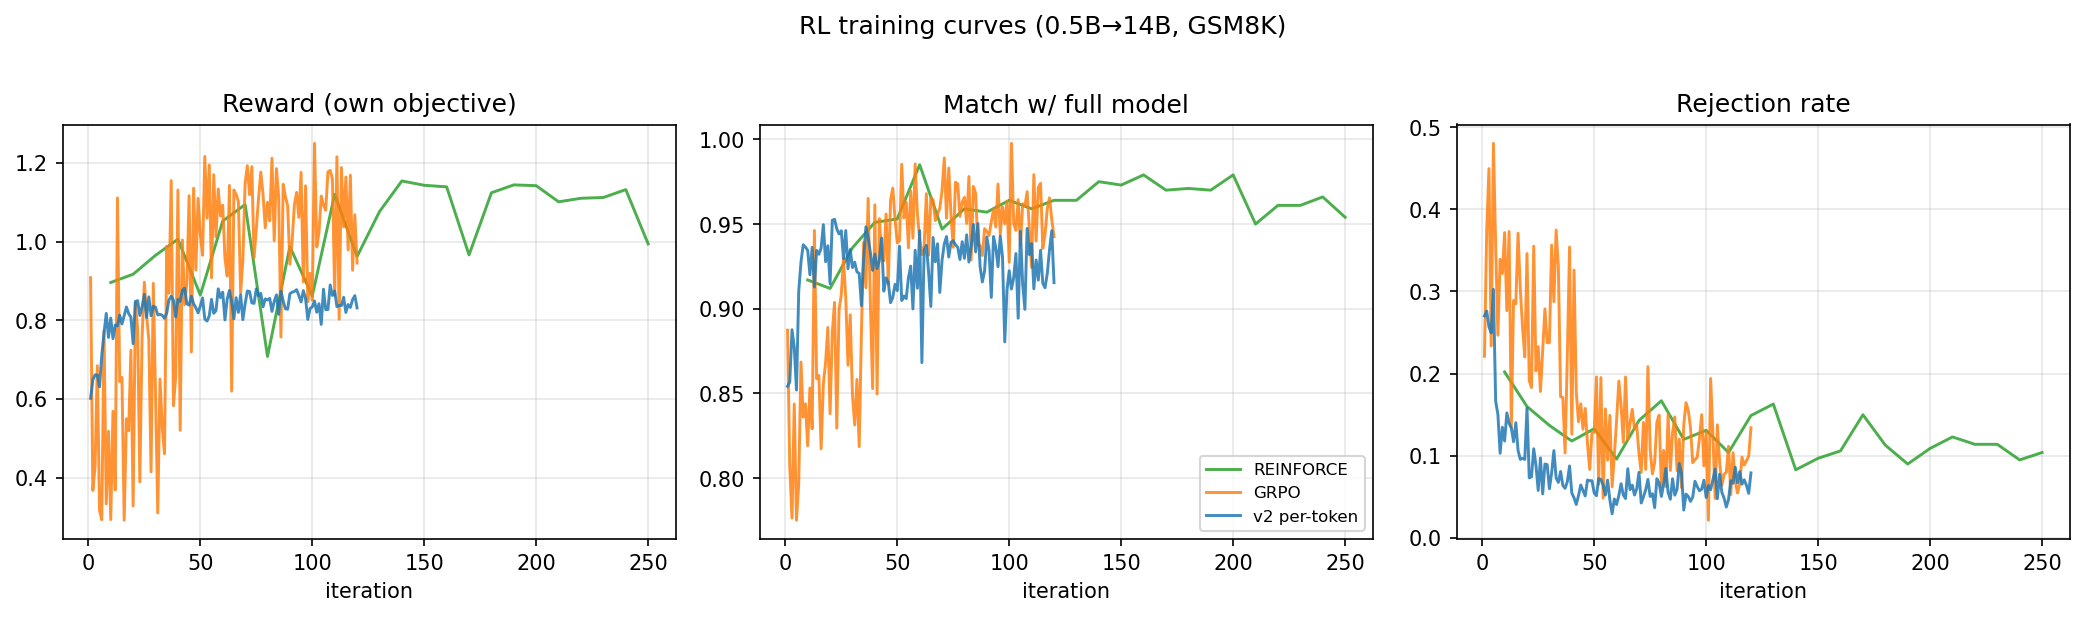
\includegraphics[width=0.9\textwidth]{results/figures/rl_curves.png}
\end{frame}
\note{
All three converge: reward up, token-match ~0.95, rejection down. The difference is variance ---
GRPO (orange) noisy, REINFORCE (green) middling, per-token v2 (blue) smoothest and lowest rejection.
Evidence for the credit-assignment point on the previous slide.
}

% =====================================================================
\begin{frame}{Results: the learned gate dominates}
\centering\small
\begin{tabular}{lccc}
\toprule
Method & GSM8K acc & q-calls/tok & speedup \\
\midrule
greedy-$q$ (reference)        & 0.887 & 1.000 & 1.00$\times$ \\
plain SD (standard, lossless) & 0.907 & 0.259 & 1.40$\times$\textsuperscript{\dag} \\
\midrule
\rowcolor{red!8} via\_fixed (paper, tuned)  & 0.40 & 0.31 & 1.76$\times$ \\
\rowcolor{red!8} via\_imit (imitation only) & 0.34 & 0.29 & 1.69$\times$ \\
\midrule
\rowcolor{blue!8} via\_rl REINFORCE          & 0.880 & 0.243 & --- \\
\rowcolor{blue!8} via\_rl GRPO               & 0.853 & \textbf{0.162} & --- \\
\rowcolor{blue!8} via\_rl REINFORCE+DIMR     & \textbf{0.907} & 0.250 & 2.22$\times$ \\
\rowcolor{blue!8} via\_rl v2 per-token       & 0.713 & 0.104 & \textbf{3.53$\times$} \\
\bottomrule
\end{tabular}
\vspace{2pt}
{\footnotesize \textsuperscript{\dag}wall-clock; via\_* speedups are the overhead-free bandwidth model (not directly comparable).}
\end{frame}
\note{
Full table. Reference at top (0.89--0.91). Red = fixed thresholds: 0.34--0.40, broken. Blue = learned
gates: REINFORCE and REINFORCE+DIMR recover full accuracy; GRPO drives expensive calls lowest (0.162);
v2 trades accuracy for top speed. Honesty note: plain SD's 1.4x is wall-clock, via\_* are an idealized
bandwidth model --- compare on q-calls/token, where the learned gates clearly win.
}

% =====================================================================
\begin{frame}{Latency: speedup by method}
\centering
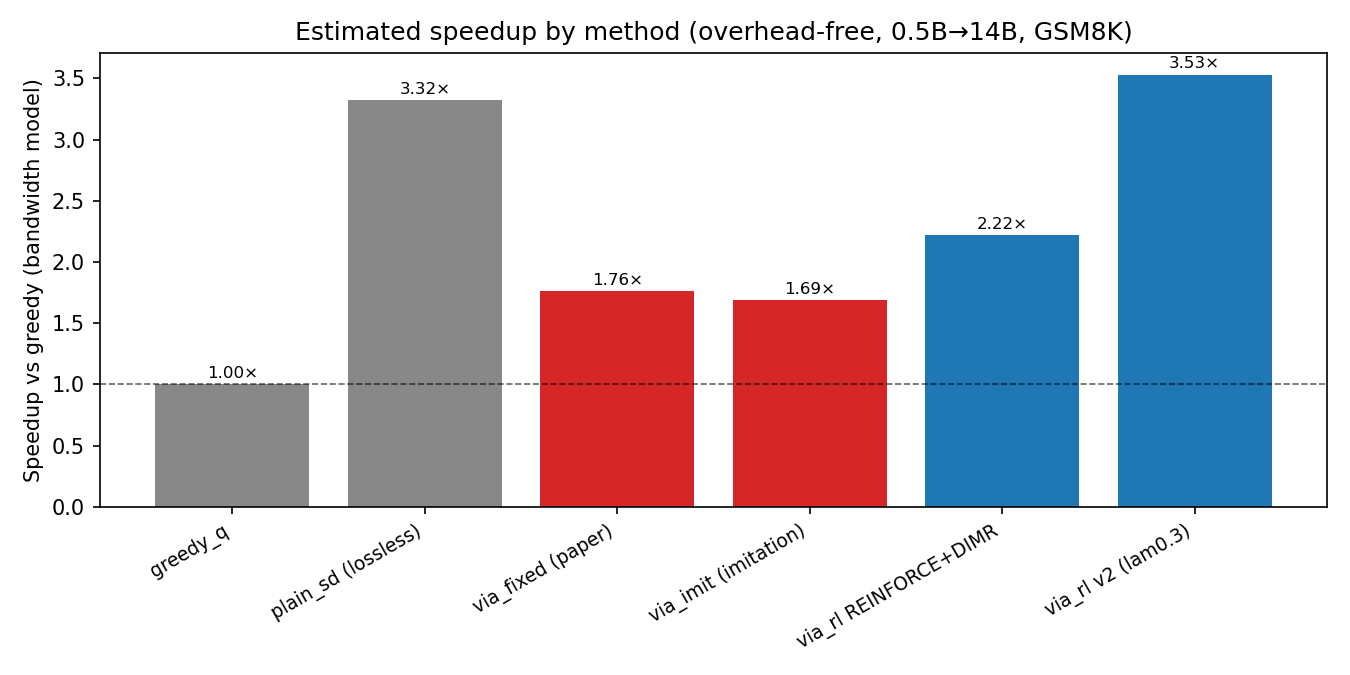
\includegraphics[width=0.8\textwidth]{results/figures/speedup_bar.png}\\
{\footnotesize plain SD = measured wall-clock; via\_* = overhead-free bandwidth model.}
\end{frame}
\note{
Greedy is the 1x baseline. The fixed-threshold gate (red) is slow --- it over-escalates. Learned gates
(blue) push speedup up; per-token v2 tops the chart by keeping escalation below break-even. Absolute
heights mix metrics (wall-clock vs bandwidth) --- the message is the ordering.
}

% =====================================================================
\begin{frame}{The accuracy--speed frontier}
\centering
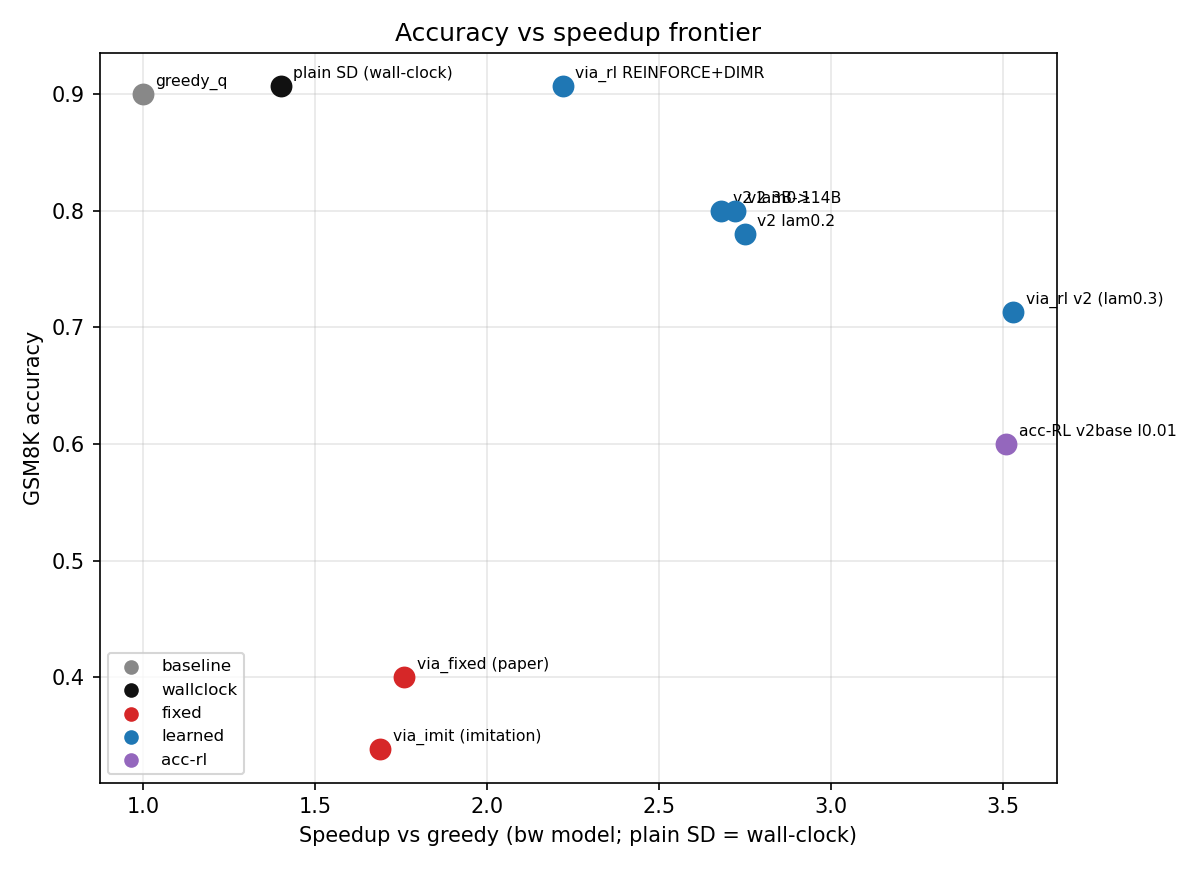
\includegraphics[width=0.6\textwidth]{results/figures/pareto.png}
\end{frame}
\note{
The design space. Red = fixed-threshold, bottom-left, dominated. Blue = learned gates, up and to the
right. The lambda knob exposes a real frontier --- accuracy (0.80) or speed (q-calls/token 0.10). And a
bigger \emph{drafter} (3B) hits 0.80 with 6x fewer verifier calls --- the right lever. The learned
policy Pareto-dominates the fixed baseline.
}

% =====================================================================
\begin{frame}{Why it matters}
\begin{itemize}
  \item We turn VIA-SD's \textbf{hand-tuned thresholds} into a \textbf{learned, per-token, context-aware} router.
  \item \textbf{Pareto-dominates} the fixed baseline; recovers \emph{lossless} quality at far fewer full-model calls.
  \item \textbf{Free to deploy:} a tiny MLP on $q$-free features --- no extra serving model, no $q$ at decision time.
  \item \textbf{Trajectory:} the gain \emph{grows} with stronger drafters --- where the field is heading.
\end{itemize}
\vspace{2mm}
\centering\textit{Stop hand-picking thresholds. Let the model schedule its own compute.}
\end{frame}
\note{
Punchline. The contribution is recognizing VIA-SD's brittle thresholds as a learnable control problem
--- and learning them. Pareto-dominates the fixed baseline, recovers lossless-level quality at a
fraction of expensive calls, and is essentially free to deploy. It improves as drafters get better,
the field's direction. Tagline: stop hand-picking thresholds; let the model schedule its own compute.
}

% =====================================================================
\begin{frame}{Future work}
\begin{itemize}
  \item \textbf{Spec-spec decoding:} make the drafter \emph{itself} speculative --- a recursive hierarchy; the gate routes across \emph{levels}.
  \item \textbf{KnapSpec:} verification as a \textbf{knapsack} --- a fixed budget of expensive calls spent on the highest-value tokens (value $=$ correctness impact, weight $=$ cost).
  \item \textbf{Correctness-floor RL:} minimize cost \emph{subject to} an accuracy floor (avoids reward-hacking collapse).
  \item \textbf{Scale:} bigger drafters, more tasks, real-engine wall-clock (static cache / CUDA graphs).
\end{itemize}
\end{frame}
\note{
Where it goes. Spec-spec: the drafter is itself slow, so make it speculative too --- a recursive tree,
gate routing across levels. KnapSpec: spend a fixed budget of expensive calls like a knapsack, on the
tokens that most change the answer --- directly targeting the match-vs-accuracy gap. Correctness-floor
RL: minimize cost subject to an accuracy floor, dodging the collapse from naive correctness rewards.
And scale it --- bigger drafters, more tasks, real wall-clock on an optimized engine.
}

\begin{frame}[plain]\centering\vfill
{\Large\textbf{Learning to Route}}\\[4pt]
Stop hand-picking thresholds --- let the model schedule its own compute.\\[8pt]
\footnotesize Thanks! \quad questions?
\vfill\end{frame}

\end{document}
